\documentclass[conference]{IEEEtran}
\IEEEoverridecommandlockouts

% ==== Fonts & core packages ====
\usepackage{newtxtext,newtxmath} % IEEE推奨Times系
\usepackage{graphicx}
\usepackage{amsmath} % amssymb は newtxmath と衝突しやすいので未使用
\usepackage{cite}
\usepackage{tikz}
\usetikzlibrary{arrows.meta,positioning,patterns}
\usepackage{xcolor}
\usepackage[hidelinks]{hyperref}

% 図の横幅を安全に抑えるヘルパー
\newcommand{\fitfig}[1]{\resizebox{0.92\linewidth}{!}{#1}}

\title{Educational Perspectives on Complementary FETs (CFET):\\
Evolution Beyond GAA and Open Challenges}

\author{
\IEEEauthorblockN{Shinichi Samizo}
\IEEEauthorblockA{Independent Semiconductor Researcher\\
Project Design Hub, Samizo-AITL\\
\textit{Email:} \href{mailto:shin3t72@gmail.com}{shin3t72@gmail.com}\quad
\textit{GitHub:} \href{https://github.com/Samizo-AITL}{Samizo-AITL}}
}

\begin{document}
\maketitle

\begin{abstract}
This tutorial paper provides an educational overview of emerging
\emph{Complementary FET (CFET)} technology, which vertically stacks nFET and pFET devices beyond Gate-All-Around (GAA) nanosheets.
CFET reframes the CMOS inverter as a \emph{cross-sectional} integration, promising density and delay improvements.
We consolidate structure, electrostatic motivations, layout and delay impacts, fabrication challenges, and modeling limitations, and articulate the pedagogical value of CFET as an open, unresolved technology for semiconductor curricula.
\end{abstract}

\begin{IEEEkeywords}
CFET, GAA, FinFET, nanosheet FET, short-channel effects, scaling, education, tutorial, vertical stacking, PDK.
\end{IEEEkeywords}

% =========================
\section{Introduction}
Scaling has progressed from planar CMOS to FinFET and most recently GAA nanosheet FETs.
Beyond the 2\,nm node, interconnect delay and cell footprint limit further gains despite excellent electrostatics.
CFET stacks nFET and pFET in the vertical dimension so that the cross-section itself constitutes a CMOS inverter, potentially doubling effective standard-cell density while shortening n--p connections.
This paper positions CFET as both a roadmap element and an educational vehicle for device--design co-optimization.

% =========================
\section{Device Evolution: From SCE Relief to Cross-Sectional CMOS}
\subsection{Planar CMOS and SCE Motivation}
As gate lengths entered the deep sub-100\,nm regime, planar MOSFETs suffered
from short-channel effects (SCE): threshold-voltage roll-off, drain-induced barrier lowering, off-state leakage, and degraded subthreshold slope.
Electrostatic control by a single top gate could no longer effectively pinch off the channel.

\subsection{FinFET: Three-Sided Gate Control}
FinFETs improved electrostatics by wrapping the gate around \emph{three} sides of a vertical fin.
The stronger gate-to-channel coupling sharpened subthreshold slope, reduced variability, and enabled higher drive per footprint by using multiple fins per device.
However, the tall/narrow fin introduced process and variability trade-offs and left one side of the channel uncontrolled.

\subsection{GAA Nanosheet: Four-Sided Control}
Gate-All-Around (GAA) nanosheet FETs extend control to \emph{four} sides by surrounding suspended sheets (or wires) with the gate.
This architecture further suppresses SCE and variability and allows continued gate-length scaling.
Yet, at advanced nodes the delay/energy bottleneck increasingly shifts from device electrostatics to \emph{wiring}: local interconnect resistance/capacitance (RC) and the lateral footprint of standard cells.

\subsection{CFET: Stacking Complementary Devices}
CFET addresses wiring and density limits by placing nFET and pFET in the \emph{same lateral footprint} and connecting them vertically.
Educational takeaways are:
(i) effective cell density can approach $\sim 2\times$ by sharing diffusion/gate footprint across polarities; and
(ii) the critical n-to-p connection in inverters and logic stacks shortens, reducing local RC and stage delay.
In short, CFET reframes CMOS as a \emph{cross-sectional inverter} rather than a lateral pair.

\begin{figure}[htbp]
\centering
\fitfig{%
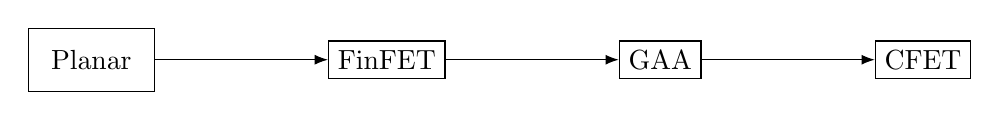
\begin{tikzpicture}[node distance=2.2cm,>=Latex]
\node[draw, minimum width=1.6cm, minimum height=0.8cm] (planar) {Planar};
\node[draw, right=of planar] (finfet) {FinFET};
\node[draw, right=of finfet] (gaa) {GAA};
\node[draw, right=of gaa] (cfet) {CFET};
\draw[->] (planar) -- (finfet);
\draw[->] (finfet) -- (gaa);
\draw[->] (gaa) -- (cfet);
\end{tikzpicture}}
\caption{Device evolution: Planar $\rightarrow$ FinFET (3-side) $\rightarrow$ GAA (4-side) $\rightarrow$ CFET (vertical stack).}
\label{fig:evolution}
\end{figure}

% =========================
\section{CFET Structural Concepts}
Two representative integration styles are considered.

\paragraph*{(i) Sequential CFET}
nFET is fabricated first, followed by pFET under a constrained thermal budget. Selective epitaxy/etch and dielectric isolation are crucial, as is vertical contact to the inverter output.

\begin{figure}[htbp]
\centering
\fitfig{%
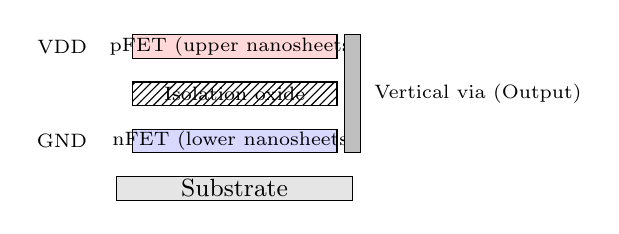
\begin{tikzpicture}[scale=1.0]
% Substrate
\fill[gray!20] (0,0) rectangle (3,0.3);
\draw (0,0) rectangle (3,0.3);
\node[font=\small] at (1.5,0.15) {Substrate};

% nFET block
\fill[blue!15] (0.2,0.6) rectangle (2.8,0.9);
\draw (0.2,0.6) rectangle (2.8,0.9);
\node[font=\scriptsize] at (1.5,0.75) {nFET (lower nanosheets)};

% Isolation
\fill[gray!35,pattern=north east lines] (0.2,1.2) rectangle (2.8,1.5);
\draw (0.2,1.2) rectangle (2.8,1.5);
\node[font=\scriptsize] at (1.5,1.35) {Isolation oxide};

% pFET block
\fill[red!15] (0.2,1.8) rectangle (2.8,2.1);
\draw (0.2,1.8) rectangle (2.8,2.1);
\node[font=\scriptsize] at (1.5,1.95) {pFET (upper nanosheets)};

% Vertical via (output)
\fill[black!25] (2.9,0.6) rectangle (3.1,2.1);
\draw (2.9,0.6) rectangle (3.1,2.1);
\node[anchor=west, font=\scriptsize] at (3.15,1.35) {Vertical via (Output)};

% Supplies (text outside to avoid overlap)
\node[anchor=east, font=\scriptsize] at (-0.25,0.75) {GND};
\node[anchor=east, font=\scriptsize] at (-0.25,1.95) {VDD};
\end{tikzpicture}}
\caption{Sequential CFET cross-section with stacked nFET/pFET and vertical output via.}
\label{fig:cfet_stack}
\end{figure}

\paragraph*{(ii) Forksheet CFET}
n/p channels are placed orthogonally with a dielectric ``fork'' spacer to ease routing congestion and preserve electrostatics.

\begin{figure}[htbp]
\centering
\fitfig{%
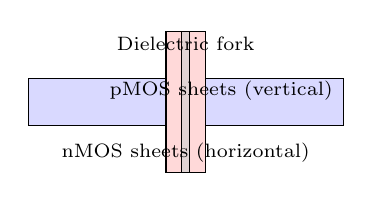
\begin{tikzpicture}[scale=1.0]
% nMOS horizontal sheets
\fill[blue!15] (0,0) rectangle (4,0.6);
\draw (0,0) rectangle (4,0.6);
% pMOS vertical sheets
\fill[red!15] (1.75,-0.6) rectangle (2.25,1.2);
\draw (1.75,-0.6) rectangle (2.25,1.2);
% dielectric fork (thin spacer)
\fill[gray!35,opacity=0.65] (1.95,-0.6) rectangle (2.05,1.2);
\draw (1.95,-0.6) rectangle (2.05,1.2);

% Labels (置き場所をずらして重なり回避)
\node[font=\scriptsize,anchor=north] at (2.0,1.25) {Dielectric fork};
\node[font=\scriptsize,anchor=south] at (2.45,0.2) {pMOS sheets (vertical)};
\node[font=\scriptsize,anchor=north] at (2.0,-0.1) {nMOS sheets (horizontal)};
\end{tikzpicture}}
\caption{Forksheet-CFET top view: orthogonal n/p nanosheets separated by a dielectric fork for routing relief.}
\label{fig:forksheet}
\end{figure}

% =========================
\section{Electrical and Layout Impacts}
Key educational points include:
\begin{itemize}
  \item \textbf{Area efficiency:} Near $\sim 2\times$ density for inverter cells; benefits extend to NAND/NOR by co-locating pull-up and pull-down networks. Standard-cell height reductions become feasible when vertical contacts are co-designed with BEOL.
  \item \textbf{Delay/energy:} Vertical n-to-p via shortens RC path; FO1 delay improves even if device $I\!-\!V$ matches GAA. Wire-limited paths in logic stacks (e.g., AOI/OAI) particularly benefit from reduced diffusion-to-diffusion distances.
  \item \textbf{Electrostatics:} Each tier can retain GAA-level control; inter-tier coupling introduces parasitics (capacitance, via resistance). Guarding isolation thickness and spacer geometry is crucial to avoid drive loss from capacitive loading.
  \item \textbf{Variability/noise:} Thermal coupling and VDD/GND partitioning introduce asymmetries requiring placement and power-routing co-optimization. Power-delivery splits (VDD top / GND bottom) alter IR drop and dynamic supply noise.
\end{itemize}

% =========================
\section{Manufacturing Challenges}
Realizing CFET integration introduces unprecedented fabrication hurdles.
Independent n/p work-functions and junctions across stacked tiers demand highly selective epitaxy and etching steps, often at low thermal budgets ($<500^{\circ}$C) to preserve the completed tier.
Alignment tolerance for vertical vias is sub-5\,nm, requiring EUV lithography overlay accuracy beyond current mass-production capabilities.
Dielectric isolation must simultaneously suppress dopant diffusion and maintain mechanical/thermal integrity across multiple layers.
Recent demonstrations by IMEC \cite{imec_cfet_iedm2020} highlight sequential CFET feasibility, but large-scale yield, variability control, and reliability remain open challenges for industry adoption.

% =========================
\section{Modeling and EDA Limitations}
Existing compact models such as BSIM-CMG \cite{bsimcmg_sispad2017} can capture GAA device behavior, but extensions to CFET remain absent.
Key missing aspects include: (i) inter-tier electrostatics, (ii) vertical thermal coupling, and (iii) parasitic R/C from stacked vias and tier-to-tier contacts.
Prototype Verilog-A implementations exist but lack consensus and calibration.
Furthermore, no open-source CFET-ready PDKs or cell libraries are available, preventing standardized design flows.
This gap not only limits immediate design enablement but also provides a fertile educational sandbox for research-oriented coursework.

% =========================
\section{Educational Value}
From a pedagogical perspective, CFET provides a unique opportunity to integrate \emph{unresolved technology} into curricula, linking physics, fabrication, and CAD.
Graduate courses can incorporate CFET Verilog-A models as design projects, explore sensitivity to inter-tier parasitics, and practice co-optimization with placement/routing.
Roadmap discussions via IRDS \cite{irds_2023} offer context for technology forecasting and design-technology co-optimization (DTCO), bridging device-level abstraction to system-level design.

% =========================
\section{Conclusion and Outlook}
CFET reframes CMOS as a stacked, cross-sectional inverter that simultaneously improves density and wiring delay.
Looking forward, forksheet layouts, sequential 3D-CFET stacks, and System-on-Stack architectures are promising research vectors.
Thermal-aware power partitioning, co-optimized BEOL integration, and AI-driven design-space exploration will be essential to reach manufacturable solutions.
Embedding CFET into curricula not only prepares engineers for the 2030s but also cultivates critical thinking about unresolved scaling frontiers.

\section*{Acknowledgment}
The author thanks the Project Design Hub community for discussions.

\bibliographystyle{IEEEtran}
\bibliography{refs}

\section*{Author Biography}
\noindent\textbf{Shinichi Samizo}
received the M.S. degree in Electrical and Electronic Engineering from Shinshu University, Japan.
He worked at Seiko Epson Corporation as an engineer in semiconductor memory and mixed-signal device development, and also contributed to inkjet MEMS actuators and PrecisionCore printhead technology.
He is currently an independent semiconductor researcher focusing on process/device education, memory architecture, and AI system integration.\\[2pt]
\textbf{Contact:} \href{mailto:shin3t72@gmail.com}{shin3t72@gmail.com}, \href{https://github.com/Samizo-AITL}{Samizo-AITL}

\end{document}
